%%      VTU Project-report Template using LaTeX
%%      
%%      Copyright 2019 vivek <vivek.adishesha@gmail.com>,
%%	keshav <keshavbharadwaj@gmail.com>
%%      
%%      This program is FREE SOFTWARE; you can redistribute it and/or modify
%%      it under the terms of the GNU General Public License as published by
%%      the Free Software Foundation; either version 2 of the License, or
%%      (at your option) any later version.
%%      
%%      This program is distributed in the hope that it will be useful,
%%      but WITHOUT ANY WARRANTY; without even the implied warranty of
%%      MERCHANTABILITY or FITNESS FOR A PARTICULAR PURPOSE.  See the\abstractintoc
\thispagestyle{plain}
\renewcommand{\abstractname}{Abstract}
\renewcommand{\abstractnamefont}{\Large\textbf}
\renewcommand{\abstracttextfont}{\normalsize}
\begin{abstract}
\OnehalfSpacing

{\LaTeX} eases our pressure in writing thesis \& reports because of its powerful features such as automatic hyphenation, table of contents, figures \& tables,  powerful bibliography tool, citations,Automatic Numbering of Chapter, sections, figures \& tables, its beautiful fonts, professional output...

Writing too much of code for gives bad impression on {\LaTeX}. But now we have numerous gui tools like gedit-latex-plugin, {\TeX}maker, Lyx \& emacs, which are very much user friendly. 

This VTU-project-report-template is written using popular document class, ``Memoir". In the coming chapters, we hav given small help manual required for writing report \& at the end about template

\end{abstract}

%%      GNU General Public License for more details.
%%      
%%      You should have received a copy of the GNU General Public License
%%      along with this program; if not, write to the Free Software
%%      Foundation, Inc., 51 Franklin Street, Fifth Floor, Boston,
%%      MA 02110-1301, USA.


%%%%%%%%%%%%%%%%%%%%%%%%%%%%%%%%%%%%%%%%%%%%%%%%%%%%%%%%%%%%%%%%%%%%%%%%%
%
\documentclass[12pt,a4paper,oneside]{memoir}%Memoir is more versatile than other document classes like article, report, book etc,
\usepackage{graphicx}%to handle image, like scaling
\usepackage[english]{babel}
\usepackage[a4paper,right=1in]{geometry}%used for modifying page layout
\usepackage{hyperref}%for referencing contents,figure,table...
\usepackage{listings}%for including source code
\usepackage{pdfpages}%to attach pdf files

%document starts here
\begin{document}
\newlength{\toptafiddle} 
\newlength{\bottafiddle}

\begin{titlingpage}
%\clearpage
\thispagestyle{empty}\centering

\setlength{\toptafiddle}{1in}
\setlength{\bottafiddle}{1in}
\vspace*{-1.25in}
\enlargethispage{\toptafiddle}
\large 
\textbf{VISVESVARAYA TECHNOLOGICAL UNIVERSITY\\
	Janana Sangama, Belgavi - 590 018}\\
\vspace{0.2cm}
\begin{figure}[h]
\centering

\includegraphics[height=3cm]{images/vtu.png}
\end{figure}
{\textbf{PROJECT REPORT ON}}\\

\Huge{\textbf{\color{red}Title of the Project}}
\vspace{0.5cm}

\large \textit{Thesis submitted in partial fulfillment for the award of degree of }{\textbf{Bachelor of Engineering}}\\
in \\\textbf{Electronics \& Communication Engineering}
\vspace{0.5cm}\\
{\textbf{Submitted by}}


\begin{tabular}{ccc}

Student-1 & \hspace{5cm}  &1RN11EC0\\
Student-2 &   &1RN11EC0\\
Student-3 &   &1RN11EC0\\
Student-4 &   &1RN11EC0\\

\end{tabular}
\vspace{0.5cm}\\
\textit{Under the Guidance of}


\Large{\textbf{Name of Guide}}\\
\textit{Designation of Guide}\\

\begin{figure}[h]
	\centering
	
\includegraphics[height=2.5cm]{images/rns1.jpg}
\end{figure}

\begin{center}
\small\textbf{DEPARTMENT OF ELECTRONICS AND COMMUNICATION ENGINEERING\\
(Accredited by NBA for the acadamic Years 2018-19, 2019-20 and 2020-21)
\\
\vspace{0.5cm}
RNS INSTITUTE OF TECHNOLOGY\\
(AICTE Approved, VTU Affiliated and NAAC 'A' credited)\\
(UG Programs - CSE, ECE, ISE, EIE and EEE have been Accredited by NBA for the Academic years 2018-19, 2019-20 and 2020-2021)\\
Channasandra,Dr.Vishnuvardhan Road,Bengaluru-560098\\
	 2019-20
}

\end{center}
\end{titlingpage}
%include titlepage,i.e, title.tex file
%Page layout according to VTU specification
%Right=1.25in,left=1in, Top & Bottom 0.75in in each

\setlength{\oddsidemargin}{0.25in}%left side margin{1in by default+0.25in}

%header specification
\setlength{\headheight}{\onelineskip}
\setlength{\headsep}{6pt}
\setlength{\topmargin}{-0.25in}

%footer specification
\setlength{\footskip}{\onelineskip}
\setlength{\footnotesep}{\onelineskip}

%A4 paper height = 11.69in
%thus 11.69in-9.67in-1in(top+header) is approx 0.75in left for bottom
\setlength{\textheight}{9.67in}

\brokenpenalty=10000% Disallow page breaks at hyphens

\OnehalfSpacing

%
\setlength{\toptafiddle}{1in}
\setlength{\bottafiddle}{1in}
\vspace*{-0.5in}
\enlargethispage{\bottafiddle}
\thispagestyle{empty}


\begin{center}
\small\textbf{	RNS INSTITUTE OF TECHNOLOGY\\
(AICTE Approved, VTU Affiliated and NAAC 'A' credited)\\
(UG Programs - CSE, ECE, ISE, EIE and EEE have been Accredited by NBA for the Academic years 2018-19, 2019-20 and 2020-2021)\\
Channasandra,Dr.Vishnuvardhan Road,Bengaluru-560098\\
\vspace{0.3cm}
DEPARTMENT OF ELECTRONICS AND COMMUNICATION ENGINEERING\\
(Accredited by NBA for the acadamic Years 2018-19,2019-20 and 2020-21)
}
\end{center}

\begin{center}
\begin{figure}[h]
\centering

\includegraphics[height=2.5cm]{images/rns1.jpg}
\end{figure}
\Large{\textbf{CERTIFICATE}}
\end{center}

Certified that thesis work entitled ``Title of the Project Report'' is carried out by Student-1, Student-2, Student-3, and Student-4 in partial fulfillment for the award of Bachelor of Engineering in Electronics \& Communication Engineering of Visvesvaraya Technological University, Belgavi, during the year 2019-2020. 


It is certified that all corrections / suggestions indicated for internal assessment have been incorporated in the report. The project report has been approved as it satisfies the academic requirements in aspect of the project work prescribed for the award of degree of Bachelor of Engineering.

\vspace{1.5cm}
\begin{minipage}[t]{0.3\textwidth}%
.......................\\
{\color{red}Name of the Guide}\\
Designation\\
\end{minipage}\hspace{0.06cm}
\begin{minipage}[t]{0.3\textwidth}%
.......................\\
{\color{red}Dr. Vipula Singh}\\
Hod\\
\end{minipage}
\begin{minipage}[t]{0.3\textwidth}%
........................\\
{\color{red}Dr. M K Venkatesha}\\
Principal\\
\end{minipage}

\begin{center}
	\textbf{{\color{blue}External Viva}}
\end{center}

\vspace{0.5cm}
\begin{minipage}[t]{0.6\textwidth}%
\textbf{Name of the examiners}\\\\
1 .....................................\\
\\
2 .....................................\\
\end{minipage}\hspace{0.06cm}
\begin{minipage}[t]{0.6\textwidth}%
\textbf{Signature with date}\\\\
.....................................\\
\\
.....................................\\
\end{minipage}

%
\setlength{\toptafiddle}{1in}
\setlength{\bottafiddle}{1in}
\vspace*{-0.5in}
\enlargethispage{\bottafiddle}
\thispagestyle{empty}


\begin{center}
\small\textbf{	RNS INSTITUTE OF TECHNOLOGY\\
(AICTE Approved, VTU Affiliated and NAAC 'A' credited)\\
(UG Programs - CSE, ECE, ISE, EIE and EEE have been Accredited by NBA for the Academic years 2018-19, 2019-20 and 2020-2021)\\
Channasandra,Dr.Vishnuvardhan Road,Bengaluru-560098\\
\vspace{0.3cm}
DEPARTMENT OF ELECTRONICS AND COMMUNICATION ENGINEERING\\
(Accredited by NBA for the acadamic Years 2018-19,2019-20 and 2020-21)
}
\end{center}

\begin{center}
\begin{figure}[h]
\centering

\includegraphics[height=2.5cm]{images/rns1.jpg}
\end{figure}
\Large{\textbf{\color{red}{DECLARATION}}}
\end{center}

We here by declare that the entire work emobodied in thsi project report titled, {\color{red}"Title"} submitted to {\color{red}Visvesvaraya Technological University}, Belagavi, is carried out by us at the department of {\color{blue}Electronics and Communication Engineering} RNS Institue of Technology, Bengaluru under the guidence of {\color{blue}Name of the Guide}, Designation. This report has not been submitted in part or full for the reward of any Diploma or degree of this or any other university.


\vspace{1.5cm}
\begin{minipage}[t]{0.4\textwidth}%

\textbf{\hspace{1.5cm}Name\\\\
1. \\\\
2. \\\\
3. \\\\
}
\end{minipage}\hspace{0.06cm}
\begin{minipage}[t]{0.4\textwidth}%

\textbf{\hspace{0.7cm}USN\\\\
1RN11EC0 \\\\
1RN11EC0 \\\\
1RN11EC0\\\\
}
\end{minipage}
\begin{minipage}[t]{0.4\textwidth}%

\textbf{\hspace{0.4cm}Signature}\\\\
.........................\\\\
.........................\\\\
.........................\\\\
\end{minipage}

\pagenumbering{roman}
\pagestyle{plain}
\renewcommand{\abstractname}{Acknowledgement}
\renewcommand{\abstractnamefont}{\Large\textbf}
\renewcommand{\abstracttextfont}{\normalsize}
\begin{abstract}
\OnehalfSpacing
%An endeavour is successful only when it is carried out under proper guidance \& blessings. We would like to thank few people who helped us in carrying out this work by lendind invaluable assistance to us in carrying out this work by lending invaluable assiatance to us.\\
%
%We are hereby thankful to Dr B.G.Sangameshwara, Principal SJCE, Mysore \& Dr C.R Venugopal, HOD of E\&C, SJCE, Mysore who encouraged at this venture
%
%We sincerely thank Dr Sudarshan Patilkulkarni, Assistant Professor Dept Of E\&C, SJCE, Mysore for constructive \& encouraging suggestions.
%
%We also thank all Teaching & Non-teaching staff of E\&C Dept SJCE, Mysore for their kind of co-operation during our course
%
%Finally we are extremely thankful to our Family \& Friends who helped us in our work \& made the project a successful one.

``\textbf{Acknowledgement} - This is where you thank all those people whom you've rarely (or never) met but whose inspiration, motivation, encouragement, blessings etc. etc. 

\vspace{3cm}
\begin{flushleft}Name1\\Name2\end{flushleft}
\vfill
\end{abstract}

\abstractintoc
\thispagestyle{plain}
\renewcommand{\abstractname}{Abstract}
\renewcommand{\abstractnamefont}{\Large\textbf}
\renewcommand{\abstracttextfont}{\normalsize}
\begin{abstract}
\OnehalfSpacing

{\LaTeX} eases our pressure in writing thesis \& reports because of its powerful features such as automatic hyphenation, table of contents, figures \& tables,  powerful bibliography tool, citations,Automatic Numbering of Chapter, sections, figures \& tables, its beautiful fonts, professional output...

Writing too much of code for gives bad impression on {\LaTeX}. But now we have numerous gui tools like gedit-latex-plugin, {\TeX}maker, Lyx \& emacs, which are very much user friendly. 

This VTU-project-report-template is written using popular document class, ``Memoir". In the coming chapters, we hav given small help manual required for writing report \& at the end about template

\end{abstract}



\setcounter{secnumdepth}{2}%sections numbering upto 2 level.i.e,chapter,section,subsection & any later sections will not be numbered
\renewcommand{\contentsname}{Table of Contents}
\tableofcontents
\newpage
\listoffigures
\newpage
\listoftables 

%creating custom header & footer. Look into memoir manual for details
\pagestyle{myheadings}
\makeheadrule{myheadings}{\textwidth}{0.4pt}
\makefootrule{myheadings}{\textwidth}{0.4pt}{\footruleskip}
\makeoddhead{myheadings}{\small{Project Title}}{}{\small{Chapter \thechapter}}
\makeoddfoot{myheadings}{\small{Dept Of E\&C, RNSIT, Bengaluru}}{}{\small{\thepage}}

\pagenumbering{arabic}

\chapter{Project}
\section{Synopsis}
\textbf{Title:} Remote servicing of IPTV using DirectFB and VNC.

\subsection{Introductory Example}
Assume you have an IPTV in your home and it has some technical problem. It will be better if the TV technician can solve the problem remotely over Internet. 

\subsection{Problem Definition}
The project involves 2 primary objectives
\begin{enumerate}
\item Exploring VNC system module of DirectFB and building it onto the target IPTV
\item Extending remote accessibility of IPTV from outside LAN
\end{enumerate}

\subsection{Existing features}
DirectFB features and VNC features have been implemented in IPTV independently.

\subsection{Our role in project}
The primary goal is establishing communication between IPTV and a remote PC for remote serviceability of IPTV.


\subsection{Hardware requirements}

\subsubsection{IPTV}
	Internet Protocol television (IPTV) is a system through which Internet television services are delivered using the architecture and networking.\cite{IPTV}\\

\subsubsection{NXP\_TV550}
	NXP\_TV550 is a single chip LCD TV platform that allows viewers to enjoy HD digital television and internet content with excellent picture quality on mid-range televisions. This module has been provided by PHILIPS and the VNC server is to be ported on this module.\\


\subsection{Software tools available}
\subsubsection{VNC}
	VNC is a remote control software which lets you see and interact with desktop applications across any network. The software has a widespread user base from individuals to the multi-national companies.You can use VNC to view a Windows 7 desktop at the office on a Linux or Mac computer at home as shown in \fref{fig:vnc} \cite{VNC}\\

\begin{figure}[h]
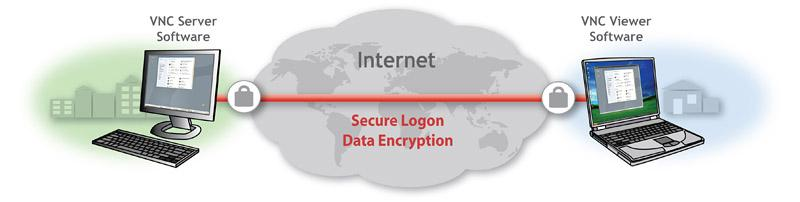
\includegraphics[scale=.5]{images/vnc.jpg}
\caption{VNC server-client model}\label{fig:vnc}
\end{figure}


\subsection{Project Organization}
	The project is split-up into 6 stages as shown in table :\\
	
\begin{tabular}{|c|c|c|}\hline
Sl No&Work& Duration(in Weeks)\\ \hline \normalsize
1&Information Collection on DFB \& VNC&1 \\ \hline
2&Information collection on development tools&2\\ \hline
3&Integrating DirectFB \& VNC&8\\ \hline
4&Cross Compiling \& Porting&2\\ \hline
5&Building JPEG libraries&2\\ \hline
6&Testing&2\\ \hline
\end{tabular}

\subsection{Project Execution}
We plan to work in these lines step-by-step
\begin{itemize}
\item Familiarize with dfb. Write simple applications. Try `windowed mode’ and `multi application mode’ on target running on X11 system module.
\item Ensure proper configuration and successful operation in these modes.
\item Run these applications on IPTV by booting from the root system on the
\item USB drive device. Control applications using putty.
\item Compile and explore fusion modules.
\item Explore vnc system module and how it provides interface options to libvnc

\end{itemize}

\include{chapter2}
\include{chapter3}
\include{chapter4}
\renewcommand{\bibname}{References}
\bibintoc %include bibliography in table of contents
\begin{thebibliography}{20}
%for books & journals
\bibitem{minix} Andrew S. Tanenbaum:\emph{Operating Systems Design and Implementation}, Prentice Hall, 2006

%for urls
\bibitem{IPTV} About IPTV on Wikipedia \url{http://en.wikipedia.org/wiki/IPTV}
\bibitem{VNC} About VNC on Wikipedia \url{http://en.wikipedia.org/wiki/Virtual_Network_Computing}
\bibitem{libvnc}LibVNC server \url{http://libvncserver.sourceforge.net}
\bibitem{dfb}DirectFB documentation \url{http://elinux.org/DirectFB}
\bibitem{jspace}jointSPACE documentation \url{http://sourceforge.net/apps/mediawiki/jointspace/index.php?title=Main_Page}
\bibitem{putty}PuTTy on Wikipedia \url{http://en.wikipedia.org/wiki/PuTTy}

%for conference papers
\bibitem{conf} Nicola L. C Talbot and Gavin C. Cawley. A fast index assignment algorithm for robust vector quantisation of image data. \emph{In Proceedings of the I.E.E.E. International Conference on Image Processing}, Santa Barbara, California, USA,  October 1997.

\end{thebibliography}


\addappheadtotoc
\begin{appendices}
\chapter{ATMega 8}%this wil by default adds Appendix A,B,C...you can specify ur own name like \chapter{Datasheets}
Here is the datasheets of various ATmega8
%\includepdf[pages=1-10]{pdf/atmega8.pdf}%here it appends only 3 pages

\end{appendices}

\end{document}
